% Created 2024-06-16 Sun 00:13
% Intended LaTeX compiler: pdflatex
ocumentclass[10pt]{article}% =================================BASE====================================%
\documentclass[10pt]{report}
\usepackage[left=2cm,right=2cm,top=2cm,bottom=2cm]{geometry} % Marges
\usepackage[T1]{fontenc} % Nécessaire avec FrenchBabel
\usepackage[utf8]{inputenc} % Important pour symboles Francophones, é,à,etc
\usepackage{csquotes} % Recommandé par PDFLatex lors de la compilation. 


% Calligraphie
%\usepackage{lmodern} % Ça, ça set latin modern
%\usepackage{mathrsfs} %Permet la command \mathscr (Lettres attachées genre) \mathscr(B)

% Calligraphie
%\usepackage{pxfonts} % Met le texte ET les maths en Palatino + donne accès à des symboles math
\usepackage{palatino} % Cette commande met seulement le texte en police palatino
\usepackage{lmodern} % Pour les maths?
% Use lmodern for sans-serif
\usepackage{mathrsfs} % Permet la command \mathscr (Lettres attachées genre) \mathscr(B)





% Bibliographie
%\usepackage[backend=bibtex,style=phys,sorting=ynt]{biblatex}
\usepackage[backend=biber,sorting=ynt,style=ieee]{biblatex}
\addbibresource{/home/charlesedouard/Desktop/Travail/Documentation/master-bibliography.bib}



\usepackage{amsmath, amssymb, amsthm} % Symb. math. (Mathmode+Textmode) + Beaux théorèmes.
\usepackage{mathtools,cancel,xfrac} % Utilisation de boîtes \boxed{} + \cancelto{}{}, xfrac
\usepackage{graphicx, wrapfig} % Géstion des figures.
\usepackage{hyperref} % Permettre l'utilisation d'hyperliens.
\usepackage{color} % Permettre l'utilisation des couleurs.
\usepackage{colortbl} % Color tables
\usepackage[dvipsnames]{xcolor} % Couleurs avancées.
\usepackage{titling} % Donne accès à \theauthor, \thetitle, \thedate

% Physique
\usepackage{physics} % Meilleur package pour physicien. 


% Style
\usepackage{lipsum} % For fun
\usepackage{tikz} % Realisation de figures TIKZ.
\usepackage{empheq} % Boite autour de MULTIPLE équations
\usepackage{bbding}

% Français
\usepackage[french]{babel} % Environnements en Français.
% ==============================BASE-(END)=================================%



% ================================SETTINGS=================================%
% Pas d'indentation en début de paragraphe :
\setlength\parindent{0pt}
\setlength{\parskip}{0.15cm}

% Tableaux/tabular
% Espace vertical dans les tabular/tableaux
\renewcommand{\arraystretch}{1.2}
% Couleur des tableaux/tabular
\rowcolors{2}{violet!5}{}

% Couleurs de hyperliens :
\definecolor{mypink}{RGB}{147, 0, 255}
\hypersetup{colorlinks, 
             filecolor=mypink,
             urlcolor=mypink, 
             citecolor=mypink, 
             linkcolor=mypink, 
             anchorcolor=mypink}


\usepackage{titling} % Donne accès à \theauthor, \thetitle, \thedate

% Physique
\usepackage{physics} % Meilleur package pour physicien. 


% Style
\usepackage{lipsum} % For fun
\usepackage{tikz} % Realisation de figures TIKZ.
\usepackage{empheq} % Boite autour de MULTIPLE équations

% Français
\usepackage[french]{babel} % Environnements en Français.
% ==============================BASE-(END)=================================%





% ================================SETTINGS=================================%
% Pas d'indentation en début de paragraphe :
\setlength\parindent{0pt}
\setlength{\parskip}{0.15cm}

% Tableaux/tabular
% Espace vertical dans les tabular/tableaux
\renewcommand{\arraystretch}{1.2}
% Couleur des tableaux/tabular
\rowcolors{2}{violet!5}{}

% Couleurs de hyperliens :
\definecolor{mypink}{RGB}{147, 0, 255}
\hypersetup{colorlinks, 
             filecolor=mypink,
             urlcolor=mypink, 
             citecolor=mypink, 
             linkcolor=mypink, 
             anchorcolor=mypink}


% Numéros d'équations suivent les sections :
\numberwithin{equation}{section} 

% Les « captions » sont en italique et largeur limitée
\usepackage[textfont = it]{caption} 
\captionsetup[wrapfigure]{margin=0.5cm}

% Retirer l'écriture en gras dans la table des matières
\usepackage{tocloft}
\renewcommand{\cftsecfont}{\normalfont}
\renewcommand{\cftsecpagefont}{\normalfont}

% Change bullet style
\usepackage{pifont}
\usepackage{enumitem}
%\setlist[itemize,1]{label=\ding{224}}
\setlist[itemize,1]{label=\ding{239}}
\renewcommand{\boxtimes}{\blacksquare}
% ================================SETTINGS=================================%



% ==============================NEWCOMMANDS================================%

% Vecteurs de base :
\newcommand{\nvf}{\vb{\hat{n}}}
\newcommand{\ivf}{\vb{\hat{i}}}
\newcommand{\jvf}{\vb{\hat{j}}}
\newcommand{\kvf}{\vb{\hat{k}}}
\newcommand{\uu}{\vb{u}}
\newcommand{\vv}{\vb{v}}
\newcommand{\ust}{\vb{u}_{\ast}}

% Physics empty spaces 
\newcommand{\typical}{\vphantom{A}}
\newcommand{\tall}{\vphantom{A^{x^x}_p}}
\newcommand{\grande}{\vphantom{\frac{1}{xx}}}
\newcommand{\venti}{\vphantom{\sum_x^x}}
\newcommand{\pt}{\hspace{1pt}} % One horizontal pt space

% Moyenne numérique entre deux points de grilles. 
\newcommand{\xmean}[1]{\overline{#1}^x}
\newcommand{\ymean}[1]{\overline{#1}^y}
\newcommand{\zmean}[1]{\overline{#1}^z}
\newcommand{\xymean}[1]{\overline{#1}^{xy}}

% Tilde over psi
\newcommand{\tpsi}{\tilde{\psi}}
\newcommand{\tphi}{\tilde{\phi}}

% Nota Bene env : (\ding{89})
%\newcommand{\nb}{$\boxed{\text{\footnotesize\EightStarConvex}\pt \mathfrak{N. B.}}$\hspace{4pt}}
\newcommand{\nb}{\underline{{\footnotesize\EightStarConvex}\pt $\mathfrak{N.B.}$\vphantom{p}}\hspace{3pt}}


% Define the nota bene environment
\usepackage{tcolorbox}
\newtcolorbox{notabene}{
     colback=blue!5,
     colframe=black,
     boxrule=0.5pt,
     arc=2pt,
     left=5pt,
     right=5pt,
     top=5pt,
     bottom=5pt,
}


\newcommand{\cmark}{\ding{52}}
\newcommand{\xmark}{\ding{55}}
% ==============================NEWCOMMANDS================================%



% ==============================PAGE-TITRE=================================%
% Titlepage 
\newcommand{\mytitlepage}{
\begin{titlepage}
\begin{center}
{\Huge Contrat Été 2023 \par}
\vspace{2cm}
{\Huge \MakeUppercase{\thetitle} \par}
\vspace{2cm}
RÉALISÉ DANS LE CADRE\\ D'UN PROJET POUR \par
\vspace{2cm}
{\Huge ISMER--UQAR \par}
\vspace{2cm}
{\thedate}
\end{center}
\vfill
Rédaction \\
{\theauthor}\\
\url{charles-edouard.lizotte@uqar.ca}\\
ISMER-UQAR\\
Police d'écriture : \textbf{CMU Serif Roman}
\end{titlepage}
}
% ==============================PAGE-TITRE=================================%



% =================================ENTÊTE==================================%
\usepackage{fancyhdr}
\pagestyle{fancy}
\setlength{\headheight}{13pt}
\renewcommand{\headrulewidth}{0.025pt} % Ligne horizontale en haut

\fancyhead[R]{\textit{\thetitle}}
\fancyhead[L]{\ \thepage}
\fancyfoot[R]{\textit{\theauthor}}
\fancyfoot[L]{}
\fancyfoot[C]{} 
% =================================ENTÊTE==================================%
\author{Charles-Édouard Lizotte}
\date{20/10/2023}
\title{Carnet de bord, Université McGill}
\hypersetup{
 pdfauthor={Charles-Édouard Lizotte},
 pdftitle={Carnet de bord, Université McGill},
 pdfkeywords={},
 pdfsubject={},
 pdfcreator={Emacs 27.1 (Org mode 9.6.7)}, 
 pdflang={French}}
\begin{document}

\mytitlepage
\tableofcontents\newpage
\section{Debuggage et implémentation transfert de masse -- \textit{<2023-10-16 Mon>}}
\label{sec:org77d1693}
\subsection{Vérifier que ce n'est pas un problème de viscosité -- \textit{<2023-10-16 Mon>}}
\label{sec:org5e06c89}
\label{org71e3432}
DEADLINE: \textit{<2023-10-17 Tue>}
Avant tout, David a remarqué que les champs de vorticité (\(\zeta_k\)) étaient extrêmement bruités, ce qui signifie qu'il y a clairement un manque à gagner en terme de viscosité.
Une viscosité plus forte permet essentiellement de se débarrasser des fluctuations aux plus petites échelles.
N'oublions pas que nous sommes passées d'une viscosité au 4ème degré vers une viscosité au second degré quand nous cherchions le problème au bord, il y a quelques semaines.
Tout ça vient confirmer ma théorie de l'escalier.\bigskip

En sommes, de nouveaux test ont été effectuées pour le schéma de viscosité exprimé par
\begin{equation}
   \vb{D} = Ah_2 \cdot \laplacian{\uu} - Ah_4\cdot \gradient^4\uu.
\end{equation}
En ce mardi matin, les résultats sont exprimés dans le tableau \ref{tab:orgec816ee}.



\begin{table}[htbp]
\caption{\label{tab:orgec816ee}Résumé des expériences réalisées dans le but de retrouver la bonne viscosité.}
\centering
\begin{tabular}{c|c|c|c|l}
\hline
Ah\textsubscript{2} & Ah\textsubscript{4} & dx & min(\sfrac{$L_d$}{dx}) & Nombre d'itér.\\[0pt]
[ -- ] & [ -- ] & [ km ] & [ -- ] & [ -- ]\\[0pt]
\hline
\hline
0.0 & (1\texttimes{}10\textsuperscript{-5})\pt\texttimes{} dx\textsuperscript{4} & 3.9 & 5.363 & 736 272 (Active)\\[0pt]
0.0 & (2\texttimes{}10\textsuperscript{-5})\pt\texttimes{} dx\textsuperscript{4} & 3.9 & 5.363 & 736 272 (Active)\\[0pt]
0.0 & (5\texttimes{}10\textsuperscript{-5})\pt\texttimes{} dx\textsuperscript{4} & 3.9 & 5.363 & 113\\[0pt]
0.0 & (1\texttimes{}10\textsuperscript{-4})\pt\texttimes{} dx\textsuperscript{4} & 3.9 & 5.363 & 48\\[0pt]
0.0 & (5\texttimes{}10\textsuperscript{-4})\pt\texttimes{} dx\textsuperscript{4} & 3.9 & 5.363 & 23\\[0pt]
\hline
\hline
\end{tabular}
\end{table}


Pour conclure, il semble que tous nos problèmes venaient bel et bien du changement de viscosité que nous avions appliqué pour régler le problème d'ondes de Kelvin aux bord (problème qui a été réglé \href{rapport-2023-10-06.pdf}{il y a deux rapports}).
Comme on peut l'observer à la figure \ref{fig:org2fe6b1f}, les \emph{eddies} sont maintenant très \emph{smooth} et non-bruités -- ce qui contraste fortement avec le dernier schéma de viscosité où l'on utilisait une viscosité au deuxième ordre plutôt qu'un viscosité avec un Laplacien d'ordre 4.
Ce qu'il faut retenir de cela c'est que le schéma utilisé dans l'article de \Textcite{chen_2021} était robuste.
Vaut mieux ne pas trop s'en éloigner. 

\begin{figure}[htbp]
\centering
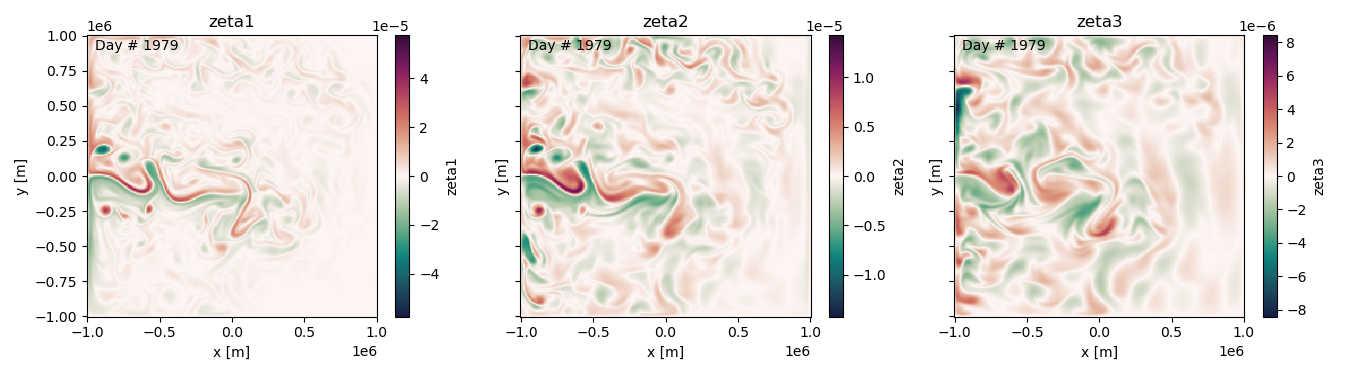
\includegraphics[width=.9\linewidth]{figures/debuggage/2023_10_17_smooth_zeta.png}
\caption{\label{fig:org2fe6b1f}Vorticité dans les trois couches après 1900 jours pour le modèle « shallow water ». On observe que les tourbillons sont très lisses dans la promière couche, en opposition au précédent schéma de viscosité utilisé.}
\end{figure}


\subsection{« Stencil » de transfert de masse -- \textit{<2023-10-23 Mon>}}
\label{sec:org9dc0cf7}
\label{orga811b83}

Louis-Philippe propose d'utiliser un stencil à 21 points pour redistribuer la masse (Voir figure \ref{org8de1f04}).
En gros, on en retirerait sur le point fautif pour rejouter du \emph{h} aux points des alentours, ce qui en fait une redistribution horizontale de la masse.\bigskip

\nb Pour l'instant (\textit{<2023-10-18 Wed>}), je met tout ça sur la glace, car la solution trouvée à la section \ref{org71e3432} semble suffisante.
Si la solution proposée à la prochaine section n'est pas suffisante, nous reviendrons sur le transfert de masse avec notre \emph{stencil}. 

\begin{figure}[!h]
\centering
\begin{tikzpicture}[scale = 0.8]
  \fill [blue!5] (1,0) -- (4,0) -- (4,1) -- (5,1) -- (5,4) -- (4,4) -- (4,5) -- (1,5) -- (1,4) -- (0,4) -- (0,1) -- (1,1) -- (1,0);
  \fill [blue!12] (1,1) rectangle (4,4);
  \draw [dotted,thin] (0,0) grid (5,5);
  \draw [] (1,0) -- (4,0) -- (4,1) -- (5,1) -- (5,4) -- (4,4) -- (4,5) -- (1,5) -- (1,4) -- (0,4) -- (0,1) -- (1,1) -- (1,0);
  \fill [cyan!50] (2,2) rectangle (3,3); 
  \draw [] (2,2) rectangle (3,3);
  %
  \draw (2.5,2.5) node {+1};
  \foreach \x in {1,2,3,4,5}{
   \draw (\x-0.5,-0.5) node {\x};
   \draw (-0.5,\x-0.5) node {\x};}
  \draw (0,5.5) node {a)};
\end{tikzpicture}\hspace{1cm}
\begin{tikzpicture}[scale = 0.8]
  \foreach \x in {-2,-1,1,2}{
   \filldraw [color=black, fill=blue!12, line width = 0.1pt] (\x,0) rectangle (\x+1,{-2*abs(1/\x)});
  }
  \filldraw [color=black, fill=cyan!50, ] (0,0) rectangle (1,3);
  \draw (0.5,1.5) node {+1};
  \draw (-2,3.5) node {b)};
  \draw (-2,0) node [left] {0};
  \foreach \x in {-2,-1,0,1,2}{
   \draw (0.5+\x,-2.5) node {\x};}
\end{tikzpicture}\hspace{1cm}
\begin{tikzpicture}[scale = 0.8]
  \fill [blue!5] (0,0) -- (3,0) -- (3,3) -- (2,3) -- (2,4) -- (0,4) -- (0,0);
  \fill [blue!12] (0,0) rectangle (2,3);
  \draw [dotted,thin] (0,0) grid (4.5,4.5);
  \draw [] (0,0) -- (3,0) -- (3,3) -- (2,3) -- (2,4) -- (0,4) -- (0,0);
  \fill [cyan!50] (0,1) rectangle (1,2);
  \draw [] (0,1) rectangle (1,2);
  \draw (0.5,1.5) node {+1};
  \draw [->, thick] (0,0) -- (5,0);
  \draw [->, thick] (0,0) -- (0,4.5);
  \draw (0,5.5) node [] {c)};
  \foreach \x in {1,2,3,4,5}{
   \draw (\x-0.5,-0.5) node {\x};
   \draw (-0.5,\x-0.5) node {\x};}
\end{tikzpicture}
\caption{\label{org8de1f04}Stencil de redistribution de la masse. À gauche (a), transfert de masse horizontal vu du haut. Au milieu (b), le même transfert de masse vu en coupe verticale. À droite (c), cas tangeant au mur.}
\end{figure}

En somme, on crée une sous-routine qui peut vérifier l'épaisseur des couches produire un transfert de masse horizontal, comme illustré à la figure \ref{org8de1f04}.
Par contre, il faudra bien faire attention lorsqu'on arrive aux murs pour que notre masque s'adapte à la forme désirée.
En ordre, les étapes à suivre sont :

\begin{enumerate}
\item On vérifie si l'épaisseur de la couche (\(h_k = H_k + \eta_k + \eta_{k+1}\)) dépasse un \emph{treshold} ou une limite verticale.
Dans notre cas, on commence à un rapport d'épaisseur de 15\% pour tester.
\item On retire l'\emph{overshoot} ( ou l'écart avec la limite \(\delta h_k\)) à la case bleue de la figure \ref{org8de1f04}.
Dans le code, c'est la quantité qu'on appelle \emph{hgap}.
\item On recrée le masque en fonction de la position par rapport aux murs.
Le poid accordé à chaque case dépend donc de la position.
\item On somme les valeurs actives du masque, de sorte à ce que le total (ou la norme) soit de 1;
\item On additionne les valeurs du masque multipliées par \(\delta h_k/2\) en haut (\(\eta_k\)) et on soustrait la même valeur en bas (\(\eta_{k+1}\)).
\end{enumerate}


\begin{figure}[h!]
\begin{center}
\begin{tikzpicture}[scale = 0.9]
\draw (-0.8,6.5) node {a)};
% Big grid
\fill [blue!5] (0,0) rectangle (3,3);
\fill [blue!5] (3,3) rectangle (6,6);
% Grid
\draw (0,0) rectangle (6,6) ;
\draw [dotted] (0,0) grid (6,6) ;
\draw [step=3.0] (0,0) grid (6,6) ;
% Carré
\fill [cyan, opacity=0.1] (2,2) rectangle (5,5) ;
\draw [cyan, thick] (2,2) rectangle (5,5) ;
\fill [cyan!50, opacity=0.5] (3,3) rectangle (4,4);
% Coordinates 
\foreach \x in {1,2,3}
\foreach \y in {1,2,3}
{\draw (\x-0.5,\y-0.5) node [] {1,1};}
%
\foreach \x in {4,5,6}
\foreach \y in {1,2,3}
{\draw (\x-0.5,\y-0.5) node [] {2,1};}
%
\foreach \x in {1,2,3}
\foreach \y in {4,5,6}
{\draw (\x-0.5,\y-0.5) node [] {1,2};}
%
\foreach \x in {4,5,6}
\foreach \y in {4,5,6}
{\draw (\x-0.5,\y-0.5) node [] {2,2};}
% Axis:
\foreach \y in {1,2,3,4,5,6} {\draw (-0.5,\y-0.5) node [cyan] {\y};}
\foreach \x in {1,2,3,4,5,6} {\draw (\x-0.5,-0.5) node [cyan] {\x};}
%
\end{tikzpicture}\hspace{1.3cm}
\begin{tikzpicture}[scale = 0.9]
\draw (-0.8,6.5) node {b)};
% Big grid
\fill [blue!7] (0,0) rectangle (2,2);
\fill [blue!7] (2,2) rectangle (4,4);
\fill [blue!7] (4,4) rectangle (6,6);
\fill [blue!7] (0,4) rectangle (2,6);
\fill [blue!7] (4,0) rectangle (6,2);
% Grid
\draw (0,0) rectangle (6,6) ;
\draw [dotted] (0,0) grid (6,6) ;
\draw [step=2.0] (0,0) grid (6,6) ;
% Carré
\fill [cyan, opacity=0.2] (1.5,1.5) rectangle (3.5,3.5) ;
\fill [cyan!50, opacity=0.5] (2,2) rectangle (3,3);
% Coordinates 
\foreach \x in {1,2,3}
\foreach \y in {1,2,3}
{\draw (2*\x-0.5,2*\y-0.5) node [] {\x,\y};
 \draw (2*\x-1.5,2*\y-0.5) node [] {\x,\y};
 \draw (2*\x-0.5,2*\y-1.5) node [] {\x,\y};
 \draw (2*\x-1.5,2*\y-1.5) node [] {\x,\y};}
% Axis:
\foreach \y in {1,2,3,4,5,6} {\draw (-0.5,\y-0.5) node [cyan] {\y};}
\foreach \x in {1,2,3,4,5,6} {\draw (\x-0.5,-0.5) node [cyan] {\x};}
%
\end{tikzpicture}
\end{center}
\caption{\label{orgd0309fb}« Stencil » utilisé pour obtenir le champs aux plus grandes échelles. À gauche (a), «stencil» pour une interoplation à ratio impair, à droite (b), «stencil» pour une interpolation à ratio pair.}
\end{figure}

\newpage
\section{Solution à la dérive de Stokes -- \textit{<2023-10-16 Mon>}}
\label{sec:org7d88a85}
Grossièrement, il est sorti deux possibilités pour régler le problème des petites échelles qui sortent de Wavewatch :
\begin{enumerate}
\item Il serait possible de diminuer la résolution de Wavewatch et de réinterpoler les points de courants à l'aide de la méthose employée dans la figure \ref{orgd0309fb}a.
Pour une interpolation \textbf{paire}, le \emph{stencil} serait un peu différent (voir figure \ref{orgd0309fb}b).

\item La seconde solution serait d'utiliser le stencil qui redistribue la masse, comme énoncé dans la section \ref{orga811b83}.
\end{enumerate}

\section{Résumé de la rencontre de mercredi [42\%]  -- \textit{<2023-10-25 Wed>}}
\label{sec:orgc174d6a}

\begin{itemize}
\item[{$\boxtimes$}] Il faut tester jusqu'à combien de couches on peut se rendre.
Bien que trois couches soit intéressant, il serait pertinent de savoir si plus de couches serait fonctionnel, maintenant que le modèle est véritablement testable.
On lance les test sans transfert de masse, considérant que c'est pas au point.\bigskip

\item[{$\boxtimes$}] Est-ce que Wavewatch est pogné avec ce \emph{fetch} là? Ça serait quand même facile de tester plusieurs \emph{switches} (voir section \ref{org5a63edf}). \bigskip

\item[{$\square$}] Un problème récurrent, c'est qu'on crée des plateaux en redistribuant la masse aux alentours.
Louis-Philippe proposait deux choses pour contrer cet effet :
\begin{enumerate}
\item \textbf{Tester un rappel plus grand} : Par exemple, à une épaisseur de moins de 15\%, on ramène tout à 15\%.
Rien ne nous oblige à ne pas ramener à 30\% et redistribuer toute cette masse-là aux alentours du point.
\item \textbf{Mettre un «threshold» plus gros} : Ça nous permettrait d'éviter que des pics d'épaisseur faible se développent dès le départ.\bigskip
\end{enumerate}

\item[{$\square$}] Les poids que j'utilise à la figure \ref{org8de1f04} sont un peu bizare.
Louis-Philippe me l'a mentionné, mais ça ne doit pas être si grave. 
\begin{enumerate}
\item \textbf{Le masque devrait être cirulaire :}
En ce moment, le masque est plutôt rectangulaire.
Louis-Philippe ne pense pas que ça soit si grave, mais tant qu'à le faire on pourrait bien le faire.
\item \textbf{Le masque n'est pas vraiment linéaire :} On rajoute une masse plus forte à côté, mais il faudrait que ça soit plus loin.
Mentionnons que je ne suis pas sur à 100\% que ça soit une bonne idée, parce que ça crérait des gradient d'épaisseurs un peu étranges.\bigskip

\nb À la rencontre du PolR, Rosalie et Jonathan ont proposé de tester plusieurs valeurs de masque ou de fenêtre.
Effectivement, la fenêtre choisie initialement donne des gros gradients d'épaisseurs qu'il faudrait peut-être modifier.\bigskip
\end{enumerate}

\item[{$\square$}] David a rappelé que la variation de l'interface pourrait devenir linéaire si on assume que \(h_k \sim H_k\).
Comme ça, ça ne changerait pas grand chose si l'épaisseur devenait nulle, mais c'est un peu une solution \emph{scotch-tape} à tester en dernier recours, selon moi.\bigskip

\item[{$\boxtimes$}] Finalement, on a un gros problème d'ordre chronologique pour adapter les épaisseurs.
Concrétement, on les modifie en même temps que trouver le \emph{RHS} des couches et des vitesses.
Il faudrait plutôt les modifier avant de calculer les \emph{RHS} associés à la vitesse et tout.
David a mentionné qu'il faut retrouver les \(\eta_k\) de la même manière qu'avec l'addition des \(RHS\ h_k\) (voir section \ref{org8919dd9}). \bigskip

\item[{$\square$}] Si rien ne marche, on peut commencer à checker pour une solution incluant un genre de Laplacien (ou de viscosité) sur les épaisseurs.
Faudra faire extrémement attention avec ça.
\end{itemize}

\section{Solutionner le chaos des vagues -- \textit{<2023-10-25 Wed>}}
\label{sec:orga6f52b7}

\subsection{Réorganiser l'ordre du transfert de masse -- \textit{<2023-10-26 Thu>}}
\label{sec:orgea28481}
\label{org8919dd9}
\textbf{Énoncé du problème :} En transférant de la masse aux niveaux adjacents, puis en calculant le \emph{RHS}, on vient modifier les épaisseurs en même temps qu'en calculant nos quantités importantes.
Essentiellement, il faut trouver un moyen de corriger toutes les épaisseurs d'un coup pour \textbf{après} calculer les \emph{RHS}. \bigskip

Concrétement, dans un boucle de \(k\) partant de la couche du haut, les étapes sont les suivantes :
\begin{enumerate}
\item On calcule l'épaisseur \(h_k\) (\emph{thickness}) et donc l'écart \emph{hgap}.
De cette manière, on trouve les positions des incursions d'eau dans les autres couches.
\item On trouve la forme horizontale (\(x,y\)) de la fenêtre (\emph{stencil}).
\item On applique le masque sur \textbf{l'interface inférieure ainsi qu'à toutes les interfaces subséquentes}.
\item On répète les étapes 1 à 3 pour les couches inférieures jusqu'à \(nz-1\).\bigskip
\end{enumerate}

\nb En additionnant la correction à toutes les couches inférieures, on s'assure que 
\begin{enumerate}
\item il n'y a pas d'overlap créé par une correction quelconque,
\item la fonction d'onde \(\psi_k\) est conservée dans les couches inférieures.
\end{enumerate}



\subsection{Tester d'autres switches pour Wavewatch -- \textit{<2023-10-26 Thu>}}
\label{sec:orgda49e8b}
\label{org5a63edf}
\begin{enumerate}
\item{$\square$} ST1,
\item{$\boxtimes$} ST2, FLX2 : Celui qu'on utilisait de base.
\item{$\boxtimes$} ST3, FLX0 : Pour vrai, ça marche mieux. La ZPPV est bien plus proche du mur et on dirait que les corrections sont moins nécessaires qu'avec ST2.
Donc, je suggère qu'on teste encore avec celle là.
\item{$\square$} ST4, \bigskip
\end{enumerate}


\subsection{Fenêtre de transfert de masse -- \textit{<2023-10-26 Thu>}}
\label{sec:org4e08c66}
Après avoir testé les \emph{switches} de la section précédentes, je vois qu'on a toujours tendance à corriger un seul point.
Ceci me laisse à penser qu'on utilise clairement une mauvaise fenêtre de transfert de masse, comme l'avait prédit Louis-Philippe et Rosalie.
Il faut donc se pencher sur ce thème-là aujourd'hui.


\printbibliography
\end{document}